\chapter{Introduction}
\label{chap:intro}
    
    \section{Phase mixing}
    \label{intro:sec:phmix}

     Weakly collisional plasmas are quite common in nature---the solar
     wind, the interstellar medium, the core of fusion devices like tokamaks being a few examples of such plasmas. Since collisions are rare,
     the particle velocity distribution functions $f(v)$ of these plasmas are not necessarily Maxwellian.
     Hence, a
     kinetic description that evolves $f(v)$  may be required to
     describe some phenomena accurately. 

	 One of
     the most important features of these systems is Landau damping, a property of
     weakly collisional plasmas whereby waves in the plasma get damped as
     non-Maxwellian structure in the distribution function is generated.  
     In his original paper, Landau \cite{landau46} considered the longitudinal
     electron oscillations \cite{tonks29} in the collisionless limit as an initial value problem, and solved it using a Laplace
     transform technique. A different approach was used by Van Kampen
     \cite{vankampen55}, in which he solved the same problem by means of a
     normal mode expansion, and found a larger set of solutions (beyond the ones that
	 satisfy the dispersion relation). Case \cite{case59} demonstrated the equivalence of these two
     approaches\footnote{He modified the Landau approach slightly, in order to derive the full set of Van
     Kampen's solutions.}, and showed that Landau damping is fundamentally a phase mixing
     process,
     %\footnote{Well known in galactic dynamics \cite{binney11}.}
     where a plane wave perturbation, written as a linear combination of the eigenmodes,
	 is damped due to the systematic smearing of the normal modes.

     \begin{figure}
     \begin{center}
        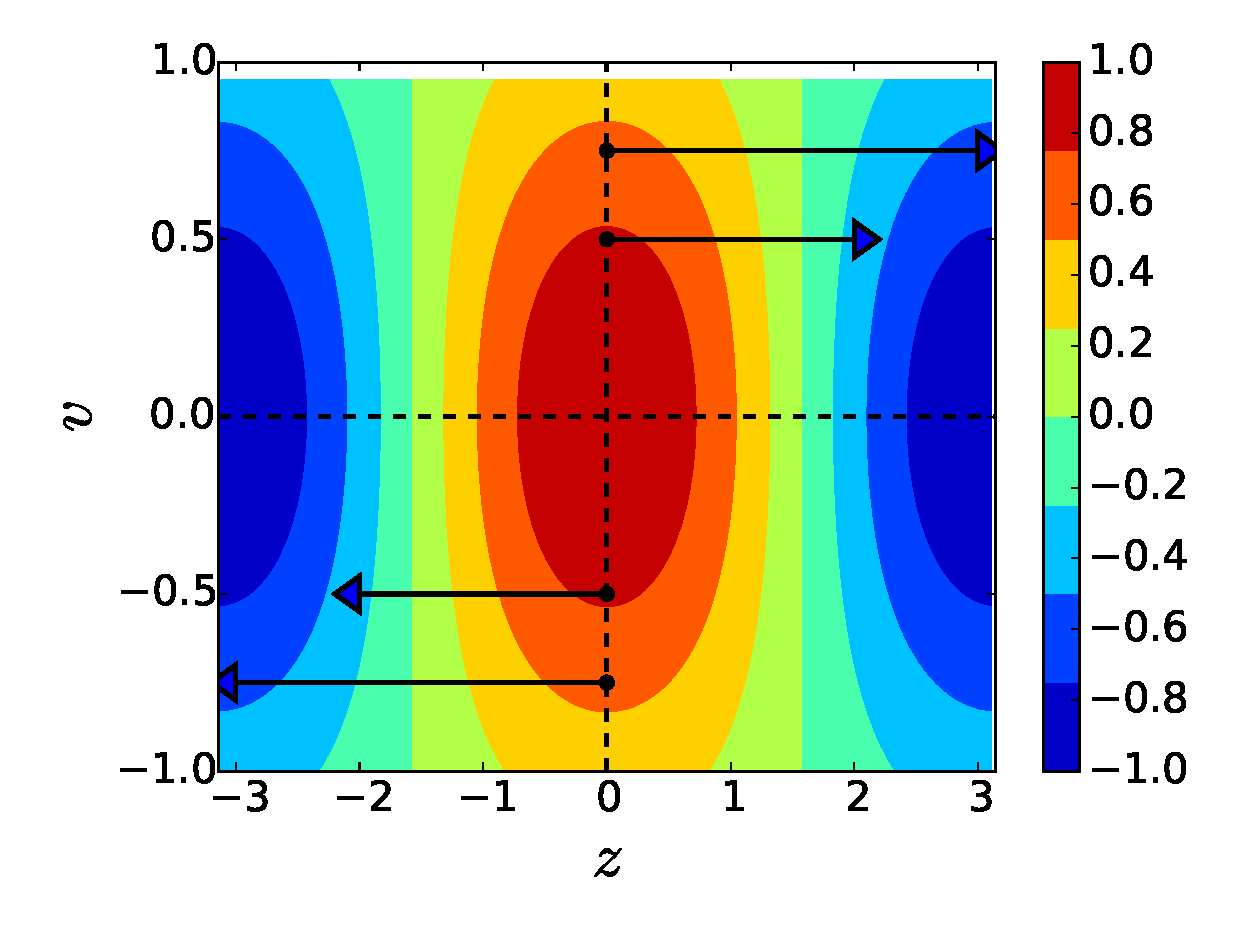
\includegraphics[width=7.4cm]{figs/intro/phmixt0.eps}
        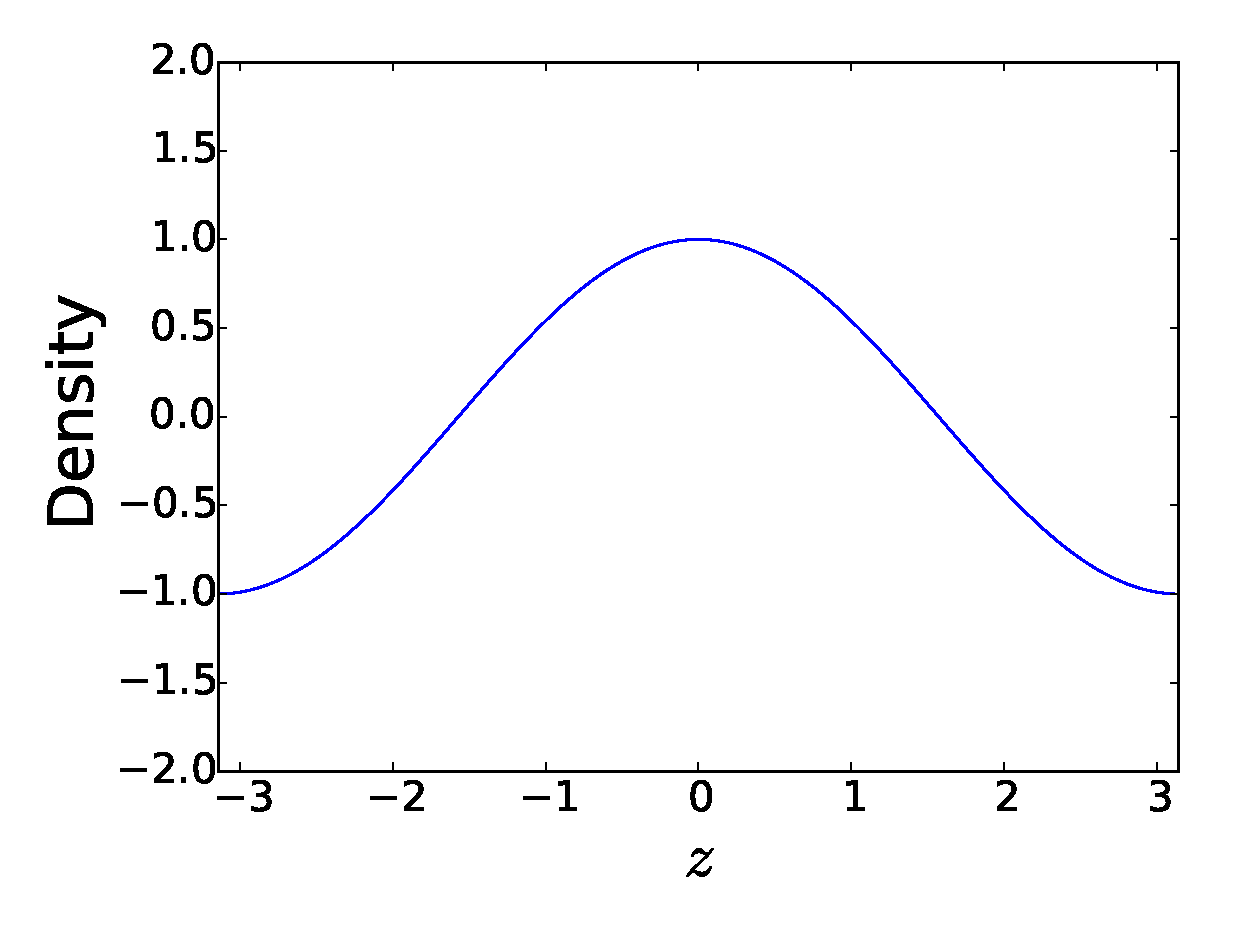
\includegraphics[width=7.4cm]{figs/intro/denst0.eps}
        \caption{The initial perturbed distribution function (left), and the corresponding density
        perturbation (right). }
        \label{intro:fig:t0}
     \end{center}
     \end{figure}

     \begin{figure}
     \begin{center}
        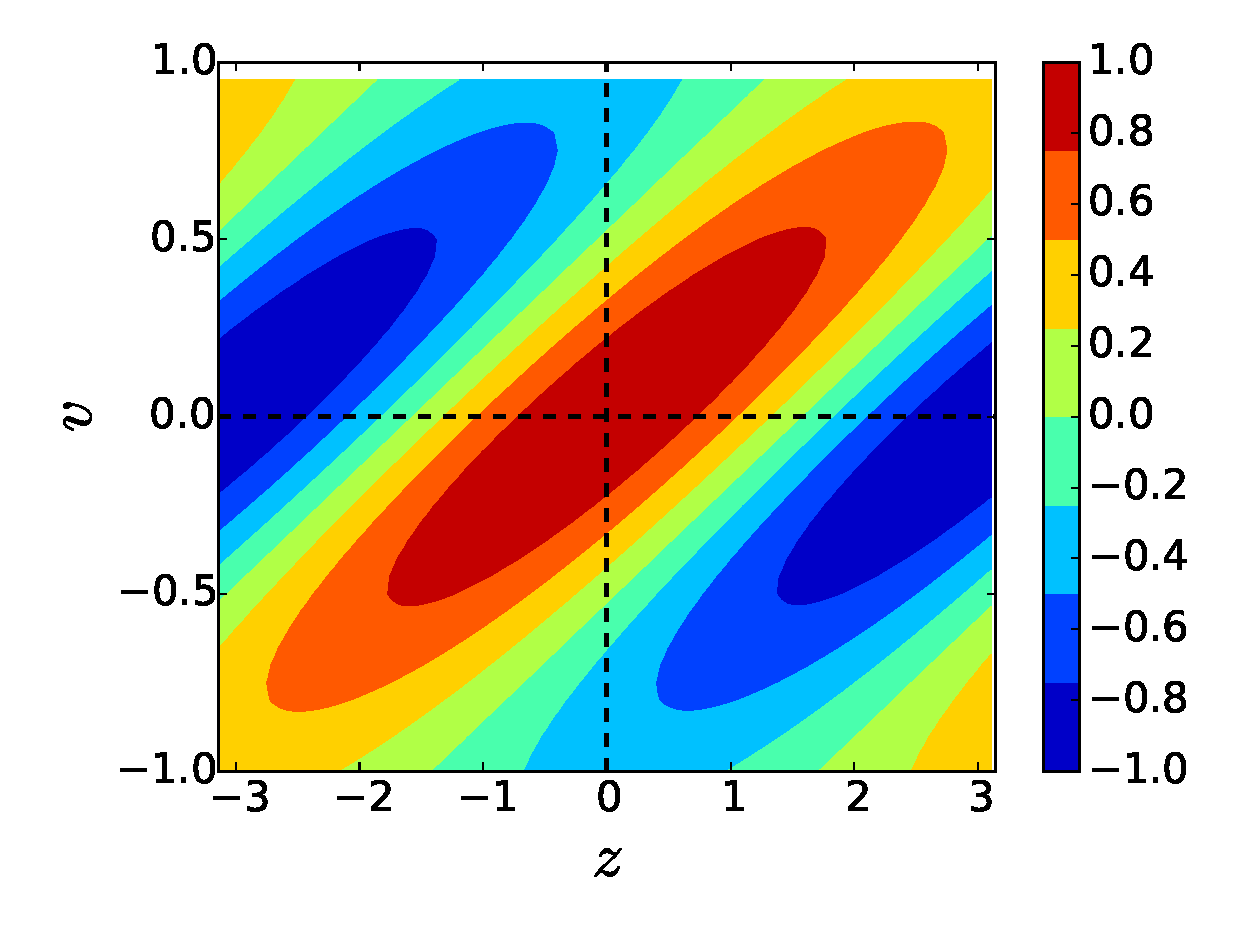
\includegraphics[width=7.4cm]{figs/intro/phmixt4.eps}
        \includegraphics[width=7.4cm]{figs/intro/denst4.eps}
        \caption{The perturbed distribution function (left), and the corresponding density
        perturbation (right) at time $t$.}
        \label{intro:fig:tt}
     \end{center}
     \end{figure}

     For a simple illustration of phase mixing, consider a
     homogeneous 1D plasma in equilibrium, with a perturbed ion distribution function
     $\delta f$: 
     \beq
        \delta f(z, v, t=0) = \cos(k z) F_0(v). \label{intro:eq:df:0}
     \eeq
     Here, the perturbation is assumed to be a cosine in the spatial direction $z$, and
     Maxwellian in velocity space, $F_0(v) = \exp\lt(-v^2/\vth^2\rt)/\sqrt{\pi}\vth$, where
     $\vth=\sqrt{2T/m}$ is the thermal velocity of the ions, $T$ is the ion temperature,
     and $m$ is the ion mass.
     This perturbed distribution function corresponds to a density perturbation $\delta n$: 
     \beq
        \delta n (z, t=0)  = \cos(k z), \label{intro:eq:dn:0}
     \eeq
     where $\delta n = \int dv\, \delta f$. The initial condition given by
     \eqsdash{intro:eq:df:0}{intro:eq:dn:0} is plotted in
     \figref{intro:fig:t0}.
     Ignoring electromagnetic effects, as time evolves, ions with different
     velocities move to different locations in space, generating structure in the
     perturbed distribution function with respect to $v$ at a
     constant $z$:
     \beq
        \delta f (z, v, t) = \cos(k z - k v t) F_0(v). \label{intro:eq:df:t}
     \eeq
     Since density is the integral of the distribution
     function over velocity ($\delta n = \int dv\, \delta f$), as the distribution function becomes more and more striated, the
     density diminishes: 
     \beq
        \delta n (z, t) = \cos(k z) \exp\lt(-k^2 \vth^2 t^2/4\rt). \label{intro:eq:dn:t}
     \eeq
     The perturbed distribution function and the perturbed density at time $t$ are plotted
     in \figref{intro:fig:tt}.
     This transfer of structure from real to velocity space, resulting in damping of low
     order velocity moments
     is known as phase mixing\footnote{There is another, nonlinear, phase mixing process
     \cite{tatsuno09}
     which plays an important role in the turbulence of weakly collisionless plasmas at scales
     comparable to the ion Larmor radius. 
      However, in
     this thesis we only consider turbulence at scales larger than the ion Larmor radius, and ignore
     this process. As a result, the linear phase mixing discussed here is the only phase mixing process in
     our models.}.

     In the collisionless limit, phase mixing is a reversible process. 
     The distribution function does not ``forget" the original perturbation that gets
     damped, and in theory, can return the system to its original state. The most famous
     example of such reversibility is the plasma echo \cite{gould67, malmberg68,
     malmberg68b, su68}. In these experiments, a perturbation of the electric potential is
     excited, which Landau damps away; later, another perturbation of the electric
     potential is excited, which also damps away; subsequently, a non-zero electric
     potential perturbation (the echo) is observed to appear in the
     plasma. The two original electric pulses couple nonlinearly to generate this echo.

     \begin{figure}
     \begin{center}
        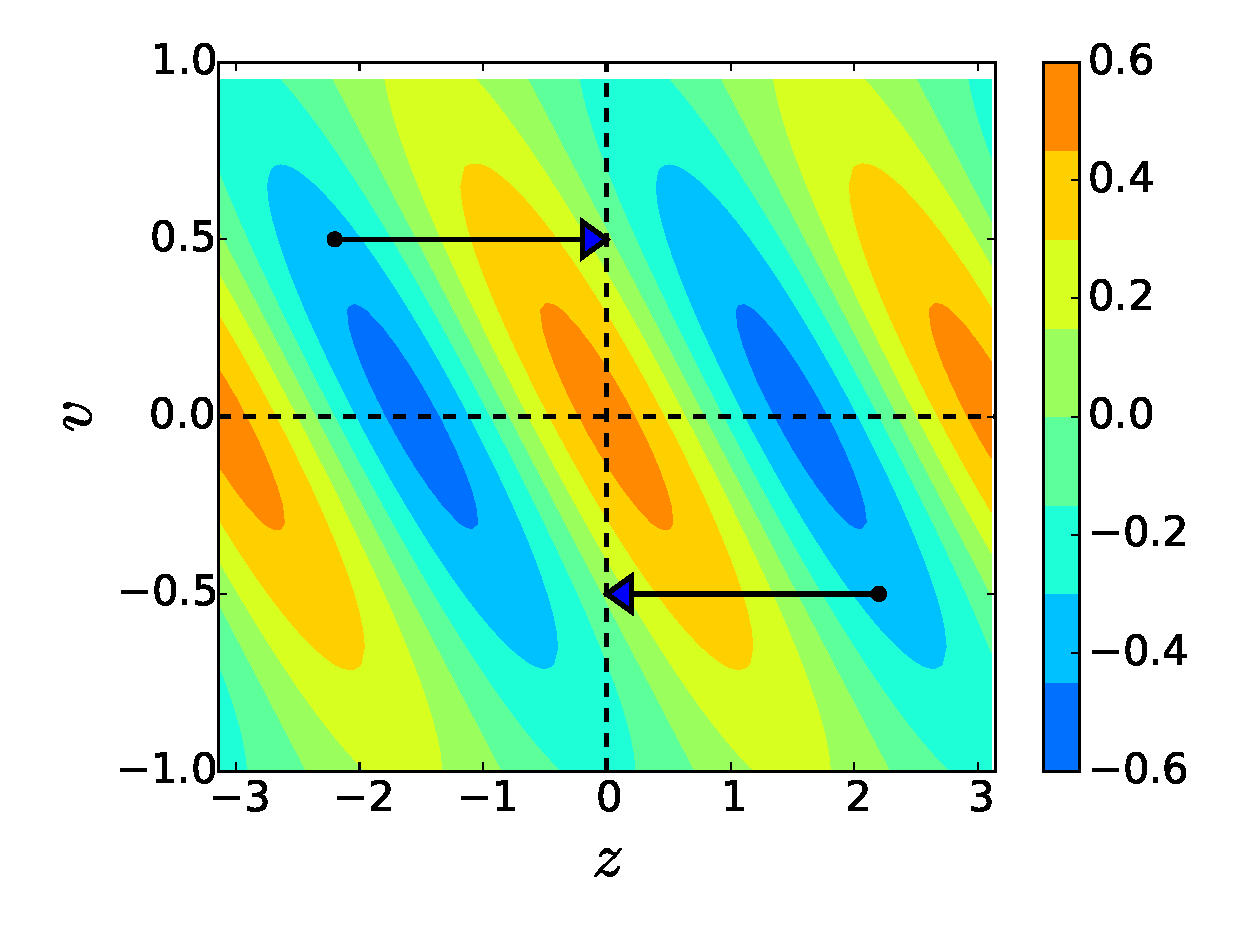
\includegraphics[width=7.4cm]{figs/intro/phmix_echot4.eps}
        \includegraphics[width=7.4cm]{figs/intro/denstecho4.eps}
        \caption{The perturbed distribution function (left), and the density perturbation
        (right), for a mode that is nonlinearly generated by the mode in
        \figref{intro:fig:tt}. It is assumed that this new mode has a wavenumber
        $p$, such that $\sgn(p) = -\sgn(k)$.} 
        \label{intro:fig:echo:t0}
     \end{center}
     \end{figure}

     \begin{figure}
     \begin{center}
        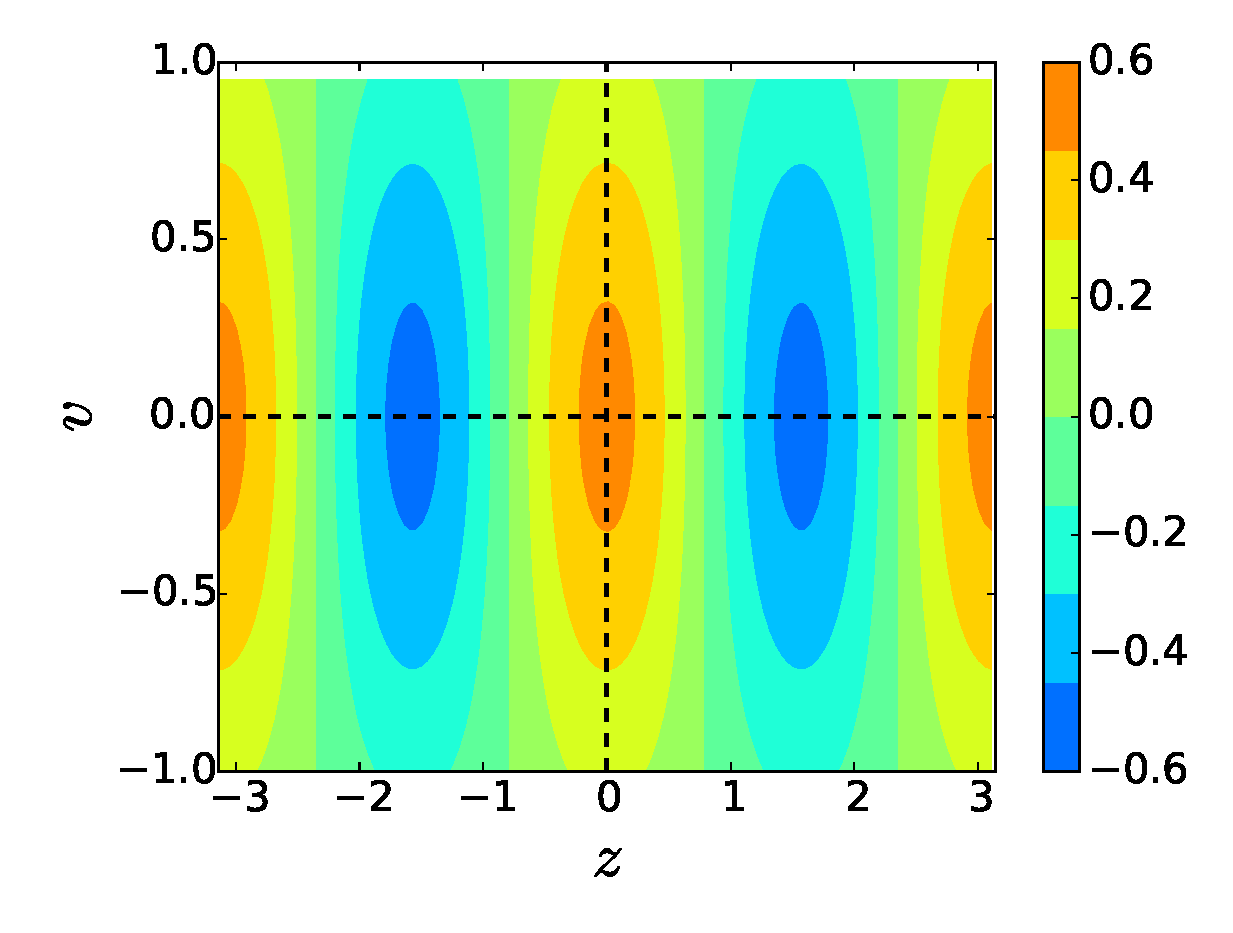
\includegraphics[width=7.4cm]{figs/intro/phmix_echot8.eps}
        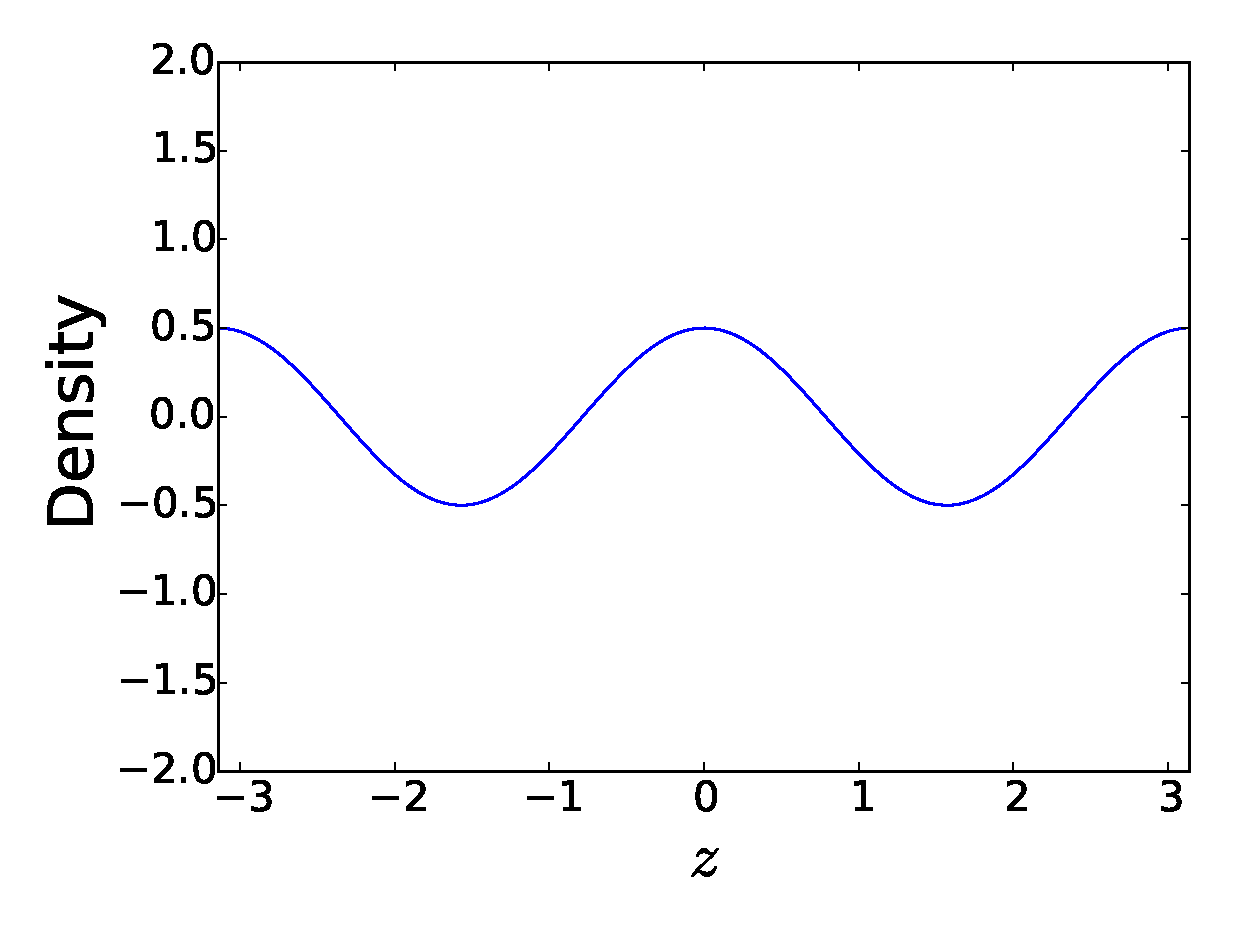
\includegraphics[width=7.4cm]{figs/intro/denstecho8.eps}
        \caption{The perturbed distribution function (left), and the density perturbation
        (right), for the mode shown in \figref{intro:fig:echo:t0}, at a later time
        $t \lt(1-k/p\rt)$.}
        \label{intro:fig:echo:tt}
     \end{center}
     \end{figure}
     
     The cartoon for phase mixing discussed above (see
     \figsand{intro:fig:t0}{intro:fig:tt}) can
     be extended to include the echo as follows.
     Imagine that the perturbation shown in \figref{intro:fig:tt} nonlinearly couples with
     another perturbation to generate
     a mode which has an oppositely signed wavenumber $p$:
     \beq
        \delta f_{\text{echo}} (z, v, t) = A \cos(p z - k v t) F_0(v),
     \eeq
     where $A$ is the amplitude of this new perturbation. This mode corresponds to a density
     perturbation given by
     \beq
        \delta n_{\text{echo}} (z, v, t) = A \cos(p z) \exp\lt(-k^2 t^2/4\rt).
        \label{intro:echo:eq:n0}
     \eeq
     The perturbed distribution function, and the density perturbation for this mode are
     plotted in \figref{intro:fig:echo:t0}. Observe that due to the change in sign of the
     wavenumber, the phase space contours of the perturbed distribution function are now tilted in the opposite way.
     At a later time $t+t'$, this perturbed distribution function evolves into
     \beq
        \delta f_{\text{echo}} (z, v, t+t') = A \cos(p z - p v t' - k v t) F_0(v).
     \eeq
     Since $p$ and $k$ are oppositely signed, the corresponding density perturbation
     at this later time is larger than the one in \eqref{intro:echo:eq:n0}:
     \beq
        \delta n_{\text{echo}} (z, v, t+t') = A \cos(p z) \exp\lt(-(kt+ pt')^2/4\rt).
     \eeq
     This perturbation is plotted in \figref{intro:fig:echo:tt} for time
     $t+t'=t\lt(1-k/p\rt)$. 
     %The generation of modes like the one shown in
     %\figref{intro:fig:echo:t0} by nonlinear interaction gives the plasma echo.

     It is shown in \chapref{chap:phmixlin} that the echo is inherently a nonlinear phenomenon, and is
     not observed for an isolated Fourier mode. In Chapters \ref{chap:pp0} and
     \ref{chap:phmixnl} nonlinear models are considered, where different Fourier modes are
     coupled to each other. Nonlinearly, the plasma echo may be observed.
     The necessary conditions required for an echo are discussed in detail within these chapters.
     

     \section{Turbulence}
     \label{intro:sec:turb}

    
    \begin{figure}
    \begin{center}
        \includegraphics[width=14.8cm]{figs/intro/turbcartoon.png}
        \caption{A cartoon picture of turbulence.}
        \label{intro:fig:turbcartoon}
    \end{center}
    \end{figure}
    Turbulence is ubiquitous, yet a precise definition of turbulence does not exist. 
	A simple picture of
	a turbulent system is depicted in \figref{intro:fig:turbcartoon}: energy is injected
	into the system at some large scale, which then cascades down to smaller and smaller
	scales. Eventually a dissipative process
	like viscosity takes over and dissipates the injected energy\footnote{\textit{Big whorls have
    little whorls that feed on their velocity, and little whorls have lesser whorls and so
    on to viscosity.}---Lewis F. Richardson}. The driving scale and
	the dissipative scale need to be far removed from each other for the system to exhibit
	turbulence. For this to be true the ratio of the driving length scale to the
	dissipation length scale, also known as the Reynolds number, is required to be large---a
    basic requirement for turbulence.

    For our purposes we broadly classify models of turbulence into two categories---fluid
    models and kinetic models. Fluid models describe systems where the mean
    free path for collisions is smaller than any length scale of interest, \ie,
    collisions are frequent. Whereas, kinetic models are applicable to systems where the
    mean free path is comparable to, or larger than the system size, \ie, collisions are
    rare. Henceforth, we use the terms ``fluid/kinetic model of
    turbulence", and ``fluid/kinetic turbulence" interchangeably.
    
    \subsection{Fluid turbulence}
    \label{intro:sec:turb:fluid}
    One of the
    first theories describing turbulence in neutral fluids was by Kolmogorov \cite{kolmogorov41},
    in which he predicts the famous $k^{-5/3}$ power law spectrum for homogeneous
    isotropic turbulence. In order to derive this spectrum, he
    made some key assumptions that have come to underlie turbulence theory: 
    \begin{inparaenum}[(i)]
        \item  statistical properties of turbulence, such as the energy spectrum, are universal at scales in between the injection and dissipation scale;
        \item the energy transfer from large to small scales happens locally in wavenumber
        space;
        \item no energy is lost at the intermediate scales, in other words, the flux of
        energy through each scale is independent of the scale.
    \end{inparaenum}

    Under these assumptions the energy density spectrum can be derived as follows: let
    $u_\lambda$ be a velocity fluctuation at the length-scale $\lambda$. The (constant) flux of energy
    $\epsilon$ through the scale $\lambda$ is then given by,
    \beq
        \frac{u_\lambda^2}{\tau_\lambda}\sim \epsilon,
    \eeq
    where $\tau_\lambda^{-1}$ is the energy cascade rate at scale $\lambda$. Since
    the energy transfer to smaller scales is local, the cascade rate must be a function
    of quantities that depend on $\lambda$. Since $u_\lambda$ and $\lambda$ are the only
    physical quantities available, the cascade rate can be estimated as,
    \beq
        \tau_\lambda \sim \frac{\lambda}{u_\lambda}.
    \eeq
    Therefore, 
    \beq
        u_\lambda^2 \sim (\epsilon \lambda)^{2/3}. \label{intro:eq:ulambda}
    \eeq
    Hence, the energy spectrum is a power law $k^{-\alpha}$. For $u_\lambda^2 \propto
    \lambda^g$, the spectral exponent $\alpha$ is calculated as $\alpha = g + 1$
    \cite{monin75}. Therefore, from \eqref{intro:eq:ulambda}, the energy spectrum for 
    turbulence in the fluid limit is $k^{-5/3}$. 
    
	The power law spectrum is characteristic of broadband fluctuations, which may
	be thought of as a signature of turbulent systems.

    \subsection{Kinetic turbulence}
    \label{intro:sec:turb:kinetic}

    \begin{figure}
    \begin{center}
        \includegraphics[width=7.4cm]{figs/intro/collisions_gas.png}
        \includegraphics[width=7.4cm]{figs/intro/collisions_plasma.png}
        \caption{Collisions in neutral fluids (left) result in sharp changes in velocity.
        Whereas, a particle (ion or electron) in a plasma undergoes many small-angle collisions
        (right). Therefore, collisions can be modeled as a diffusive operator in the
        velocity co-ordinate.}
        \label{intro:fig:collisions}
    \end{center}
    \end{figure}
    In this section, we shall move away from the discussion about neutral fluid turbulence, and discuss the
    general properties of turbulence in weakly collisional plasmas.
    In addition to the fluid-like turbulent cascade in real space, weakly collisional
    systems also allow for   
    transfer of energy to small velocity space scales by phase mixing. This makes the nature
    of dissipation for such systems a contentious issue \cite{parashar13}.
	Even though phase mixing damps
    perturbations in the plasma, the process is reversible in the
	collisionless limit, \ie, it does not generate 
	entropy. Therefore, phase mixing is not dissipative in the true sense. Irreversible heating for these systems is only possible through collisions
	\cite{schekochihin08, tome}. Collisions in plasmas are of a different character than
    the ones in neutral fluids (see \figref{intro:fig:collisions}). Unlike neutral fluids,
    particles (ions or electrons) in a plasma undergo numerous long-range collisions, which
    individually do not
    alter the velocity of the particle by much. 
	Therefore, collisions can be modeled as a diffusive operator in velocity space: $\sim \nu \,
	\partial_v^2$ \cite{howes06, tome}, where $\nu$ is the frequency with which a particle velocity is changed by
    $\pi/2$ radians. For systems with vanishingly
	small $\nu$, energy has to be transferred to small scales in velocity space, before it
    can dissipate via collisions. As a result, in the weakly collisional limit, the cascade of energy
    occurs in the phase space (real and velocity space) \cite{schekochihin08, tome,
    tatsuno09}---the spatial cascade is the usual fluid-like nonlinear refinement of
    scales, whereas the cascade in velocity space is due to phase mixing.
    
    The systems studied in this thesis are assumed to be weakly collisional, and allow for 
    the above mentioned phase space cascade. 

\section{Magnetized plasmas}

    In addition to assuming that the plasma is weakly collisional, it
    is also assumed to be strongly magnetized. A strongly magnetized plasma is threaded by
    a mean magnetic field such that the ion Larmor radius is much smaller than the system
    size. Additionally, it is assumed that
    the magnitude of the background magnetic field is much larger than the turbulent electromagnetic fluctuations. For
    magnetic confinement fusion devices, this is a given, as a guide field is necessary for
    confinement of the burning plasma. For space and astrophysical plasmas, the large scale
    magnetic fluctuations behave as a background magnetic field for the small scale
    turbulence (Kraichnan hypothesis \cite{kraichnan65}). 

    The background magnetic field makes these systems very anisotropic \cite{goldreich95,
    goldreich97}---the
    perpendicular length scales ($\lambda$) are much smaller than the parallel length
    scales ($l$). For such anisotropic systems, the Kolmogorov derivation for the energy spectrum is no longer
    possible, since the timescale at a given scale cannot be determined uniquely. There
    is a perpendicular, nonlinear timescale $\lambda/u_\lambda$, and a parallel,
    linear timescale associated with the Alfv\'{e}n waves $l/v_A$,
    where $v_A$ is the Alfv\'{e}n velocity. In the magnetohydrodynamic limit, Goldreich and Sridhar \cite{goldreich95,
    goldreich97} proposed a way forward by assuming that the turbulence, at sufficiently
    small scales, arranges itself in such a way that the linear and nonlinear
    timescales are comparable to each other \cite{galtier00, schekochihin12}. This assumption, taken scale by scale is
    known as \textit{critical balance}. One can then estimate the cascade time as
    \beq
        \tau_\lambda \sim \frac{\lambda}{u_\lambda} \sim \frac{l}{v_A},
    \eeq
    which once again gives,
    \beq
        u_\lambda \sim (\epsilon \lambda)^{1/3}.
    \eeq
    This again corresponds to a $k_\perp^{-5/3}$ spectrum, but now the spectrum is in the
    perpendicular direction, as opposed to the isotropic spectrum derived earlier for neutral
    fluids.
    The critical balance
    assumption also relates the parallel and perpendicular length scales:
    \beq
        l \sim l_0^{1/3}\lambda^{2/3}, \label{intro:eq:critanis:l}
    \eeq
    where $l_0 = v_A^3/\epsilon$; $l_0$ is the parallel length scale where the velocity
    fluctuation is comparable to the Alfv\'{e}n velocity, and can be thought of as a
    natural outer scale. Therefore, the velocity fluctuation scaling with respect to $l$
    is given by 
    \beq
        u_\lambda \sim \lt(\frac{\epsilon^{1/3}}{l_0^{1/6}}\rt) l^{1/2}.
    \eeq
    This corresponds to a parallel spectrum of
    $\kpar^{-2}$. The relationship given by \eqref{intro:eq:critanis:l} between the parallel and
    perpendicular length scales looks like $\kpar~\sim~k_\perp^{2/3}$ in terms of the
    wavenumbers, \ie, as the cascade moves forward to smaller spatial scales, it gets
    increasingly anisotropic.

    In addition to the spatial scale separation, the background magnetic field also
    separates timescales. The cyclotron motion may be assumed to be much faster than any
    timescale of interest in
    the system---this allows for reduced descriptions of kinetic plasmas, which are
    discussed further in \secref{intro:sec:krmhd} and \apref{app:eq}.

\section{Phase mixing in turbulent magnetized plasmas: Questions}
    
    In \secsand{intro:sec:phmix}{intro:sec:turb} we discussed how phase mixing
    and turbulent cascade dictate the turbulent characteristics of a plasma individually. It is
    however unclear, as to
    what happens to phase mixing in a nonlinear turbulent system. Understanding how phase
    mixing works in presence of turbulence is an important problem in kinetic plasma
    turbulence.

     \begin{figure}
     \begin{center}
        \includegraphics[width=7.4cm]{figs/intro/Armstrong_dens.jpg}
        \includegraphics[width=7.4cm]{figs/intro/solarwind_dens.jpg}
        \caption{Density fluctuation spectra in the interstellar medium (left, taken from
        \cite{armstrong95}) and the solar wind (right, taken from \cite{marsch90}). These power law
        spectra span multiple decades, even at scales where these fluctuations are
        expected to be strongly damped.}
        \label{intro:fig:dnespec}
     \end{center}
     \end{figure}

    A simple way to incorporate phase mixing in a model for a turbulent plasma 
    would be to introduce it as
    a sink of energy to small velocity
    scales, at each spatial scale, in essence superimposing phase mixing
    on to the turbulent cascade \cite{quataert98, quataert99, howes08jgr}. For the cascade of a macroscopic quantity like
    density fluctuations, this would show up as a scale-by-scale dissipative term, where the rate of
    dissipation is proportional to the parallel wavenumber. 
    Such dissipation would violate the constant-flux-through-scales assumption of
    Kolmogorov. Extraction of energy at each scale at a rate proportional to
    the wavenumber
    would imply that the energy spectrum 
    should be an exponential decay instead of a power law.
    However, power law energy spectra are commonly observed in weakly collisional turbulent
    magnetized plasmas.
    A striking example is that of compressive
    fluctuations in astrophysical systems. Electron density
    fluctuations in the interstellar medium extend over twelve decades of scales, 
    famously known as ``the Great Power Law in the Sky" \cite{armstrong81, armstrong95,
    lazio04}. In the solar wind, these
    fluctuations are observed for roughly three decades \cite{lovelace70, woo79, celnikier83,
    celnikier87, coles89, marsch90, coles91, bershadskii04, hnat05, kellogg05,
	alexandrova08} (see \figref{intro:fig:dnespec}). These observations are at scales
    where the plasma is weakly collisional. Linear theory predicts that compressive
    fluctuations should be strongly damped in the weakly collisional limit \cite{barnes66}, which makes
    these observed power law spectra surprising.
    This suggests that when the system is nonlinear, the linear predictions need to be
    modified.
    A possible explanation for such power law spectra, though not specifically for these
    plasmas, was given recently by Plunk \etal\
    \cite{plunk13, plunk14}, where they argue that phase mixing is suppressed due to
    what is in essence, an ``impedance mismatch" with the nonlinear turbulent frequency.
	However, in
    their study, they do not include the nonlinear cascade. Instead, they consider a
    single Fourier mode, and add a random source term as a stand-in for
    turbulence---this approach is quite different from the one we adopt here.

    In this thesis, the interplay between the nonlinear cascade and phase mixing is
    studied.
    This is done by considering nonlinear models which incorporate both these effects\footnote{This is different from what is generally referred to as nonlinear
    Landau damping (see \cite{mouhot11} and references therein for a detailed analysis of
	this problem from a mathematician's perspective) in the literature. The question there
	is what happens to the validity of Landau's results
    if the perturbations have finite amplitudes. In our work, all perturbations are
    assumed small compared to the equilibrium.}.
%     In chapter \ref{chap:phmixlin}, we analytically derive the behavior of a
%     driven-damped system in absence of
%    turbulent cascade. In chapters \ref{chap:pp0} and \ref{chap:phmixnl}, we consider 
%    simple models of kinetic passive scalar turbulence, where we discuss the fate of phase
%    mixing in the presence of turbulent cascade. In
%    \chapref{chap:slowmodes}, we present results from direct numerical simulations of
%    compressive fluctuations in the solar wind, and describe a possible mechanism that
%    would explain the observed power law spectra for density and field strength
%    fluctuations at kinetic scales (\figref{intro:fig:dnespec}). The numerical tool developed for this work
%    is described in \chapref{chap:gandalf}.
%    
%    It is important to understand what happens to phase
%    mixing in presence of turbulence in order to address this discrepancy.
%    At this point it is important to mention that 
%    ``Landau fluid" models\cite{hammett90, hammett92, hedrick92, dorland93, beer96,
%    snyder97, snyder01, snyder01gf, passot04, ramos05, goswami05, passot06, passot07,
%    passot12}, though more sophisticated in nature, use the same basic
%    principle of extracting energy from higher velocity moments at the linear damping
%    rate. These models have shown tremendous success in reproducing experimental results
%    for fusion plasmas, and seem to be generally used in scenarios where phase mixing
%    remains essentially unaltered due to turbulence.
%
%
    The first nonlinear model allows for a turbulent cascade in the direction
    perpendicular to the guide field, but does not allow for a transfer of energy to small
    spatial scales parallel to the background field. In this scenario, when the turbulent
    cascade rate is comparable to or larger than the phase mixing rate, energy gets swept up
    to small spatial scales before it can phase mix. As a result a fluid-like turbulent
    cascade, \ie\, a power law spectrum is observed. In the other, more interesting model, where the turbulent cascade
    proceeds in both perpendicular and parallel directions, 
    a turbulent analog
    of the plasma echo is observed, which unravels the velocity space structure generated by
    phase mixing. This
    \textit{stochastic plasma echo} suppresses phase mixing, which again results in a fluid-like
    turbulent cascade at scales where, in the linear limit, perturbations would be
    strongly damped due to phase mixing. Hence, regardless of whether or not there is a
    parallel cascade, power law energy spectra are observed for
    turbulent fluctuations at these ``kinetic" scales.
    
    \section{Kinetic Reduced MHD}
    \label{intro:sec:krmhd}
    \subsection{Basic framework}
    
    The basic mathematical framework used in this work is
    known as Kinetic Reduced MagnetoHydroDynamics (KRMHD). KRMHD is the
    long wavelength limit of gyrokinetics \cite{rutherford68, taylor68, catto78, antonsen80,
    catto81, frieman82, dubin83, lee83, lee87, hahm88, howes06, tome}. It is derived in
    thorough detail in Schekochihin \etal\ \cite{tome}, by expanding ``$\delta f$ gyrokinetics"  in small $k_\perp \rho_i$ ($k_\perp$ is the perpendicular wavenumber,
    $\rho_i$ is the ion Larmor radius). In this limit, the Alfv\'{e}nic component of
    the cascade
    decouples from the compressive fluctuations. The dynamics of the system are completely
    determined by the Alfv\'{e}nic fluctuations, which evolve according to reduced MHD
    \cite{kadomtsev74, strauss76}. The compressive
    fluctuations, on the other hand, are described by a kinetic equation for a passive
    scalar that is nonlinearly advected by the background Alfv\'{e}nic turbulence. These
    equations provide an efficient framework within which one may study the turbulent cascade
    of density and field strength fluctuations in weakly collisional turbulent magnetized
    plasmas like the solar wind. 
    
    The passive nature of compressive fluctuations in this
    model neatly ties in with a popular approach used to study turbulent cascade in fluid
    systems, namely that of passive scalar turbulence \cite{obukhov49, corrsin51, batchelor59,
    kraichnan68, kraichnan74, kraichnan94,
    monin75, aref84, chaiken87, ottino89, zeldovich88, ott88, ott89, antonsen91, ramashankar91,
    solomon93, sreenivasan91,
    vanatta91, pierrehumbert94, antonsen95, frisch95, sreenivasan96, boratav97, lesieur97, shraiman00,
    warhaft00}. This gives us the opportunity to study the general problem of
    \textit{kinetic} passive
    scalar turbulence, while having a physically relevant system to compare with.
    General results regarding kinetic passive scalar turbulence are presented in Chapters
    \ref{chap:phmixlin}, \ref{chap:pp0} and \ref{chap:phmixnl}, by considering simplified
    versions of KRMHD. The full KRMHD equations are
    numerically solved in \chapref{chap:slowmodes}.

    The derivation of KRMHD given in Schekochihin \etal\ \cite{tome} is extremely detailed, and we
    do not attempt to better it in this thesis. Instead, we give an outline of the
    derivation of KRMHD in \apref{app:eq}, and give a summary of the final equations here.
    
    The KRMHD model assumes a homogeneous equilibrium, with a Maxwellian as the background
    distribution function. A perturbation of this equilibrium is evolved in time. 
    The Alfv\'{e}n cascade is described by reduced MHD,
    which in its simplest form is written in terms of Elsasser variables \cite{elsasser50}:
    \beq
    \pd{\nabla_\perp^2 \xi^\pm}{t} \mp v_A \pd{\nabla_\perp^2 \xi^\pm}{z} = - \frac{1}{2} \left[
    \{\xi^+, \nabla_\perp^2 \xi^- \} + \{\xi^-, \nabla_\perp^2 \xi^+ \} \mp \nabla_\perp^2
    \{\xi^+, \xi^-
    \} \right], \label{intro:krmhd:els} 
    \eeq
    where the background magnetic field $\mb{B}_0 = B_0\hat{\mb{z}}$ is in the
    $\hat{\mb{z}}$ direction, $\hat{\mb{x}}$ and $\hat{\mb{y}}$ are the transverse directions,
    $\xi^\pm = \Phi \pm \Psi$, $v_A = B_0/\sqrt{4 \pi m_i n_{0i}}$ is the Alfv\'{e}n
    velocity, and $\Phi$ and $\Psi$ are stream and flux functions
    respectively, which are related to the electrostatic potential ($\phi$) and the magnetic vector
    potential ($\Apar$) by:
    \beq
        \Phi = \frac{c}{B_0}\phi, \quad \Psi = - \frac{\Apar}{\sqrt{4 \pi m_in_{0i}}}
        \label{intro:eq:PhiPsi},
    \eeq
    where $c$ is speed of light,
    $m_i$ is the ion mass, and $n_{0i}$ is the background ion density.
    The braces denote the Poisson bracket:
    \beq
        \lt\{P,Q\rt\} = \pd{P}{x}\pd{Q}{y} - \pd{P}{y} \pd{Q}{x}.
    \eeq

    The left hand side of \eqref{intro:krmhd:els} describes Alfv\'{e}n wave packets,
    traveling up or down the field line. The nonlinear interaction between these wave
    packets is captured by
    the right hand side. Observe that only counter-propagating Alfv\'{e}n waves interact
    nonlinearly; these counter-propagating Alfv\'{e}n waves give rise to the turbulent cascade by
    transferring energy to smaller spatial scales.

    The compressive fluctuations are described in terms of two Elsasser-like variables
    $g^+$ and $g^-$:
    \beq
    \od{g^\pm}{t} + \vpar \nabla_\parallel g^\pm  = \frac{\vpar F_0(\vpar)}{\Lambda^\pm}
    \hat{\mb{b}}\cdot\nabla \int d \vpar g^\pm, \label{intro:krmhd:gpm}
    \eeq
    where $F_0(\vpar)=\exp(-\vpar^2/\vth^2)/\sqrt{\pi} \vth$ is a one-dimensional
    Maxwellian ($\vth=\sqrt{2T_i/m_i}$ is the thermal velocity of ions, $T_i$ is the ion
    temperature, $m_i$ is the ion mass), and
    \beq
        \Lambda^\pm = -\frac{\tau}{Z} + \frac{1}{\beta_i} \pm \sqrt{\lt(1 +
        \frac{\tau}{Z}\rt)^2 + \frac{1}{\beta_i^2}}, \label{intro:krmhd:Lambda}
    \eeq
    where $\tau$ is the ion to electron temperature ratio, $Z$ is the ion charge in units
    of the electron charge, and $\beta_i = 8\pi n_{0i} T_i/B_0^2$ is the ion plasma beta.
    We observe from \eqref{intro:krmhd:Lambda}, that the range of $\Lambda^\pm$ is
    restricted to: $\Lambda^+ > 1$, and $\Lambda^- < 0$. The derivatives $d/dt$ 
    and $\nabla_\parallel$ in \eqref{intro:krmhd:gpm} are convective derivatives:
    \beq
        \od{}{t} = \pd{}{t} + \lt\{\Phi,\ldots\rt\}, \quad \nabla_\parallel =
        \pd{}{z} + \frac{1}{v_A}\lt\{\Psi,\ldots\rt\}.\label{intro:krmhd:convder}
    \eeq
    The relationship between
    the perturbed ion distribution function and $g^\pm$ is given in \apref{app:eq} (see
    \eqsand{eqs:eq:gnBdef}{eqs:krmhd:gpmdef}).
%These are in fact described 
%by two equations evolving two decoupled 
%functions $g^+$ and $g^-$, which are certain linear combinations 
%of the zeroth and second moments of the perturbed ion distribution 
%function with respect to the velocity perpendicular to the 
%mean magnetic field (taken to be in the $z$ direction). 
%These equations are derived in \cite[][\S 6.2.1]{tome} 
%and are of the form \exref{phmixlin:eq:g} with 
%\beq
%\alpha^\pm =-\lt[-\frac{T_i}{ZT_e} + \frac{1}{\beta_i}\pm A\rt]^{-1}, \quad
%A = \sqrt{\lt(1+\frac{T_i}{ZT_e}\rt)^2 + \frac{1}{\beta_i^2}} 
%\eeq
%for $g^\pm$, respectively (here $\beta_i=8\pi n_iT_i/B^2$ is the ion beta). 
%The physical fields, the density and magnetic-field-strength perturbations, are related 
%to $g^\pm$ by 
%\begin{align}
%\frac{\delta n}{n} &= \frac{1}{2A}\int\rmd v\lt[\lt(1 + \frac{T_i}{ZT_e} + \frac{1}{\beta_i} + A\rt)g^-
%- \frac{T_i}{ZT_e}\frac{2}{\beta_i}\,g^+\rt],\\
%\frac{\delta B}{B} &= \frac{1}{2A}\int\rmd v\lt[\lt(1 + \frac{T_i}{ZT_e} + \frac{1}{\beta_i} + A\rt)g^+
%- \lt(1+\frac{ZT_e}{T_i}\rt)g^-\rt].
%\end{align}
%While these expressions are perhaps not very physically transparent, it may aid 
%intuition to note that ${\delta n}/{n} \approx \int\rmd v g^-$ and 
%${\delta B}/{B} \approx \int\rmd v g^+$ either in the limit of 
%high $\beta_i$ and hot ions ($T_i\gg T_e$) or in the limit of 
%low $\beta_i$ and cold ions ($T_i\ll T_e$). At low $\beta_i$, the $g^-$ equation 
%describes ion-acoustic waves ($\alpha^-\approx ZT_e/T_i$; see above). 
%At high $\beta_i$, the $g^+$ equation describes a kinetic version of the MHD slow mode, 
%subject to a version of Landau damping due to \cite{barnes66}; 
%in this case, $\alpha^+\approx -1 + 1/\beta_i$. 
%
    \Eqsand{intro:krmhd:els}{intro:krmhd:gpm} together constitute the KRMHD model.

    \subsection{Conserved quantities}
    \label{intro:sec:krmhd:const}


    The energies in each of the Elsasser variables ($\xi^\pm, g^\pm$) are conserved
    independently in KRMHD:
    \beq
        W = W_{\text{AW}}^+ + W_{\text{AW}}^- + W_{\text{compr}}^+ + W_{\text{compr}}^-,
    \eeq
    where 
    \beq
        W_{\text{AW}}^\pm = \int d^3\mb{r} \frac{m_i n_{0i}}{2}
        \lt|\nabla_\perp\xi^\pm\rt|^2
    \eeq
    are energies of the right and left-going Alfv\'{e}nic fluctuations, and
    \beq
        W_{\text{compr}}^\pm = \int d\mb{r}\frac{n_{0i}T_{0i}}{2}\lt[\int d\vpar
        \frac{\lt(g^\pm\rt)^2}{F_0} - \frac{1}{\Lambda^\pm}\lt(\int d\vpar
        g^\pm\rt)^2\rt] \label{intro:eq:Wcomp}
    \eeq
    are energies of the $+$ and $-$ components of the compressive
    fluctuations\footnote{Both the terms in \eqref{intro:eq:Wcomp} are positive for
    the ``$-$" mode, since $\Lambda^- < 0$. For the ``$+$" mode, $W_{\text{compr}}^+$ can be
    shown to be positive using Cauchy-Schwarz inequality, and the condition $\Lambda^+>1$.}, as
    defined in the previous section, respectively; $W$ is the total free energy.

